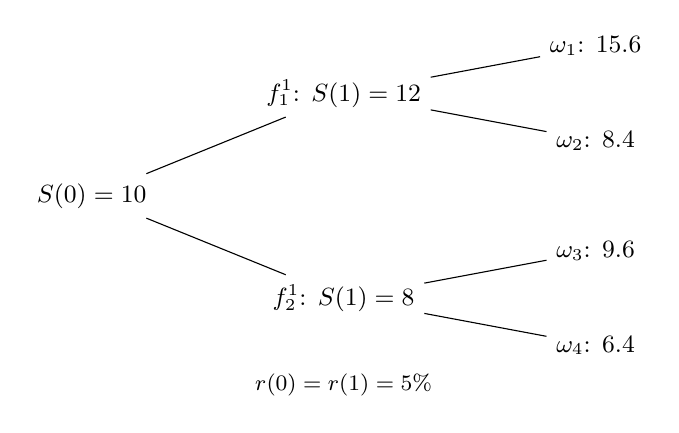
\begin{tikzpicture}[grow=right,level 1/.style={level distance=3.2cm,sibling distance=2.6cm},level 2/.style={level distance=3.2cm,sibling distance=1.2cm},every node/.style={font=\small}]
\node{$S(0)=10$}
 child{node{$f^1_2$: $S(1)=8$} child{node{$\omega_4$: $6.4$}} child{node{$\omega_3$: $9.6$}}}
 child{node{$f^1_1$: $S(1)=12$} child{node{$\omega_2$: $8.4$}} child{node{$\omega_1$: $15.6$}}};
\node[font=\footnotesize] at (3.2,-2.4) {$r(0)=r(1)=5\%$};
\end{tikzpicture}
